\chapter{評価}
本章では,本研究で開発した個人認証システムのパラメータ調整と調整後の識別精度,登録及び認証処理にかかる時間の評価を行う.
なお,パラメータ調整と識別精度の評価を行うために,事前に本システムを用いてあらかじめ6名の被験者に端末を持ち上げるモーションを4回入力してもらい,モーションデータの収集を行った.
また,なりすまし認証のモーションデータとして,筆者自身が同様のモーションを入力して得たモーションデータを用いた.

% 各種パラメータの変更による識別率の変化もまとめる
% @suppress
\section{識別器のパラメータ調整}
本システムの識別器におけるDenoising Autoencoderの次元削減率とダミーデータのダミー割合を決めるため,2名の被験者から得たモーションデータを用いて識別器の出力を確認しつつ調整を行った.
Denoising AutoencoderのDropout率やノイズ割合は一般的な推奨値とされる50\%と30\%を設定した.
学習回数と許容誤差はパラメータ調整時の誤差の縮小度合いをモニタリングした結果と,現実的な時間で学習処理が終わることを考慮し,Denoising Autoencoderでは200回と0.1を,識別器では500回と0.1を設定した.
また,調整時になりすまし認証のモーションデータも入力し,被験者のモーションデータを入力した際には識別器の出力値が低く,なりすまし認証のモーションデータを入力した際には識別器の出力値が高くなるようなパラメータを調べた.

パラメータ変更に伴う被験者Aと被験者Bの出力値の変化と,なりすまし認証の出力値をまとめたものを付録\ref{tune-a}と付録\ref{tune-b}にそれぞれ示す.
表における行が次元削減率,列がダミー割合を示している.
% 10/40, !20/40, !40/40, !50/20, ok50/30, !60/30, 80/50, 90/80
この結果から,被験者のデータによる出力が0.5以下でなりすまし認証のデータによる出力が0.5以上,かつ次元削減率が50\%前後という条件で識別率の良かった,次元削減率が50\%でダミー割合が30\%という組み合わせを本システムで採用した.

% @suppress ParagraphNumber JapaneseAmbiguousNounConjunction InvalidSymbol
\section{識別精度の評価}
各被験者ごとに,あらかじめ収集したモーションデータの最初の3回分を登録モードにおける学習データ,最後の1回分を認証モードにおける入力データとして,識別器の学習と識別を10回ずつ試行して識別精度の評価を行った.
また,それぞれの試行時になりすまし認証データも入力した.

\begin{table}[btph]
  \centering
  \caption{識別精度の評価結果}
  \label{auth-result}
  \begin{tabular}{|c|r|r|r|r|r|} \hline
    回数 & 1 & 2 & 3 & 4 & 5 \\ \hline
    A & 0.303649 & 0.297174 & 0.103238 & 0.27233 & 0.286347 \\
    なりすまし & 0.99843 & 0.999783 & 1 & 0.999994 & 1 \\ \hline
    B & 0.410452 & 0.541679 & 0.393484 & 0.498285 & 0.402412 \\
    なりすまし & 0.390929 & 0.954446 & 0.714886 & 0.986832 & 0.771009 \\ \hline
    C & 0.463514 & 0.535742 & 0.429281 & 0.431916 & 0.660576 \\ % refresh c, d, e, f
    なりすまし & 0.511741 & 0.57337 & 0.585036 & 0.40849 & 0.897041 \\ \hline
    D & 0.542743 & 0.469785 & 0.478641 & 0.206191 & 0.316994 \\
    なりすまし & 0.51709 & 0.790494 & 0.860314 & 0.665402 & 0.366732 \\ \hline
    E & 0.369962 & 0.775177 & 0.930394 & 0.620721 & 0.861707 \\
    なりすまし & 0.425681 & 0.622781 & 0.823906 & 0.322503 & 0.808092 \\ \hline
    F & 0.427885 & 0.480025 & 0.526025 & 0.398201 & 0.602788 \\
    なりすまし & 0.440998 & 0.57856 & 0.40198 & 0.756612 & 0.580305 \\ \hline \hline
    回数 & 6 & 7 & 8 & 9 & 10 \\ \hline
    A & 0.230282 & 0.377003 & 0.460634 & 0.519086 & 0.286327 \\
    なりすまし & 1 & 1 & 1 & 1 & 1 \\ \hline
    B & 0.592374 & 0.602627 & 0.465201 & 0.389765 & 0.426538 \\
    なりすまし & 0.970552 & 0.977083 & 0.53193 & 0.809484 & 0.765663 \\ \hline
    C & 0.316001 & 0.409446 & 0.456424 & 0.319418 & 0.221473 \\
    なりすまし & 0.32995 & 0.843308 & 0.667239 & 0.332062 & 0.489108 \\ \hline
    D & 0.558527 & 0.410008 & 0.458197 & 0.429079 & 0.503082 \\
    なりすまし & 0.662734 & 0.77522 & 0.502198 & 0.630231 & 0.637029 \\ \hline
    E & 0.895046 & 0.834229 & 0.527374 & 0.738395 & 0.989204 \\
    なりすまし & 0.431249 & 0.790342 & 0.612434 & 0.649207 & 0.778007 \\ \hline
    F & 0.474251 & 0.31154 & 0.592163 & 0.391282 & 0.49657 \\
    なりすまし & 0.518223 & 0.235919 & 0.578955 & 0.389576 & 0.658209 \\ \hline
  \end{tabular}
\end{table}

この実験により識別器から得られた出力をまとめたものを表\ref{auth-result}に示す.
全体的に見ると,被験者のモーションデータとなりすまし認証によるモーションデータで出力に差ができており,上手く識別できているように見える.
だが,被験者Fの3回目の試行のように,他の試行では上手く識別できたにもかかわらず失敗しているものがある.
また,被験者Eについてはほぼ全ての試行でなりすまし認証のモーションによって得られた値が被験者のモーションデータによって得られた値を下回っている.

本システムでは端末所有者のモーションデータとなりすまし認証によるモーションデータを識別するために,識別器の学習時に端末所有者のモーションデータのほかに,データの30\%を0で上書きしたダミーデータを用いた.
元データに0に近い値が多く含まれる場合は0で上書きしてもあまり違いが出ないことから,また元データの次元数が少ない場合は上書きするデータ数が少ないことから,元データとの差があまり出ない可能性がある.
これにより,端末所有者が入力したモーションデータであってもなりすまし認証であると識別されてしまったのではないかと考えられる.

また,モーションデータの入力回数毎にデータのばらつきが多く一致している部分があまりなかった場合,識別器の学習が進まず,上手く識別できなくなる可能性も考えられる.
識別率の良かった被験者Aのモーションデータを図\ref{comp-a}に,良くなかった被験者Eのモーションデータを図\ref{comp-e}に示す.

\begin{figure}[bthp]
  \centering
  \begin{tabular}{c}
    \begin{minipage}{.48\hsize}
      \centering
      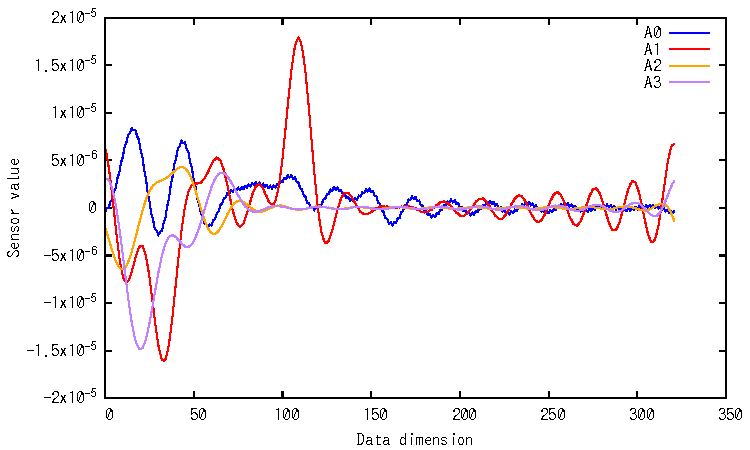
\includegraphics[bb=0 0 360 216, width=8cm]{Graphs/comp_A.pdf}
      \caption{被験者Aのデータ}
      \label{comp-a}
    \end{minipage}
    \begin{minipage}{.48\hsize}
      \centering
      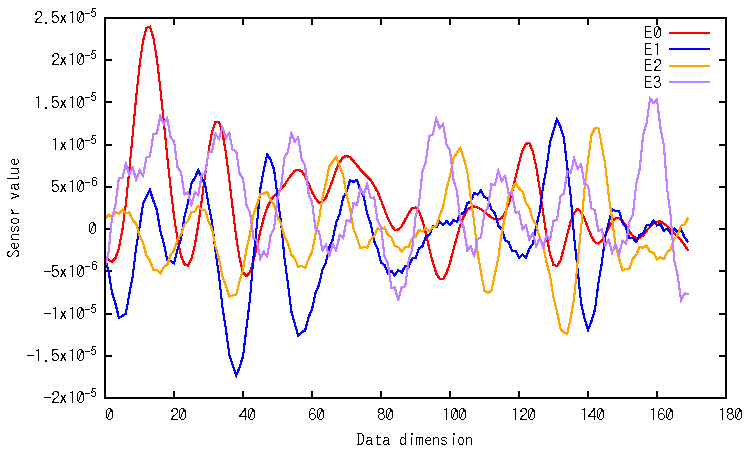
\includegraphics[bb=0 0 360 216, width=8cm]{Graphs/comp_E.pdf}
      \caption{被験者Eのデータ}
      \label{comp-e}
    \end{minipage}
  \end{tabular}
\end{figure}

\section{登録及び認証の処理時間の評価}
本システムについて,登録及び認証の処理時間を計測した.
Androidのログ出力用APIとして用意されているLogクラス\cite{5-log}を用い,モーション入力が終了し計算処理中であることをユーザに示すプログレスダイアログが表示される部分と,登録及び認証処理が終わり処理結果が表示される前にプログレスダイアログが非表示となる部分にログ出力を行うコードを挿入した.
このログから出力される時刻情報から処理時間を求めて評価を行った.
また,認証モードについては端末内での計算処理も行えるため,こちらの処理時間も求めることとする.

評価の結果,サーバを用いた場合の登録処理ではおよそ38秒,認証処理ではおよそ2秒となった.
また,端末内での認証処理ではおよそ2.2秒となった.

ただし,モーションデータの次元数が多い場合や,サーバを多数のユーザが利用する場合はより長い処理時間を要すると考えられる.
